%%%%%%%%%%%%%%%%%%%%%%%%%%%%%%%%%%%%%%%%%%%%%%%%%%%%%%%%%%%%%%%%%%%%%%%%%%%%%%%%%%
\begin{frame}[fragile]\frametitle{}
\begin{center}
{\Large Deep Learning in NLP}

\tiny{(Ref: Deep Learning and NLP A-Z - Kirill Eremenko)}
\end{center}
\end{frame}

%%%%%%%%%%%%%%%%%%%%%%%%%%%%%%%%%%%%%%%%%%%%%%%%%%%%%%%%%%%
\begin{frame}[fragile]\frametitle{What is Deep NLP}
\begin{center}
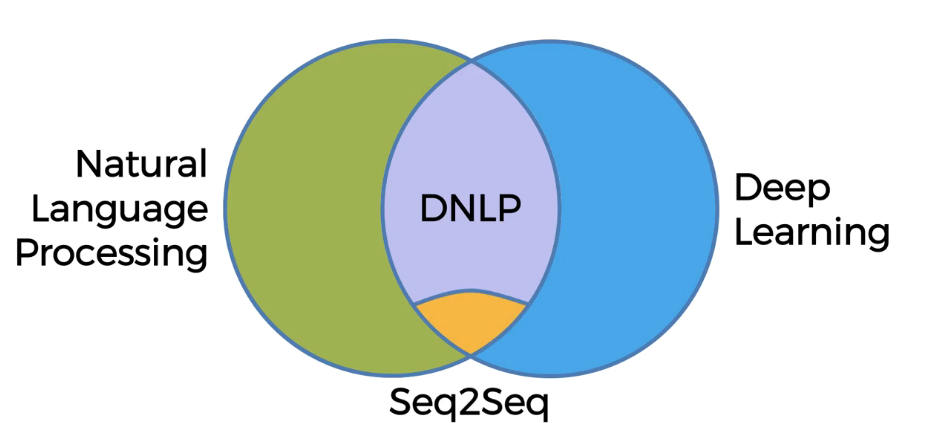
\includegraphics[width=0.8\linewidth,keepaspectratio]{nlp4}

\tiny{(Ref: Deep Learning and NLP A-Z - Kirill Eremenko)}

\tiny{(Note: Size is not indicative of importance)}
\end{center}

	\begin{itemize}
	\item Green part is NLP (rule based, linguistic)
	\item Blue part is Deep Learning not applied to NLP
	\item Purple is Deep NLP (DNLP), NN applied for NLP use cases
	\item Seq2Seq is heavily used technique of DNLP for sequence to sequence modeling, eg Translation, Q \& A, etc.
	\end{itemize}
	

\end{frame}

%%%%%%%%%%%%%%%%%%%%%%%%%%%%%%%%%%%%%%%%%%%%%%%%%%%%%%%%%%%
\begin{frame}[fragile]\frametitle{Traditional vs Deep NLP}
\begin{center}
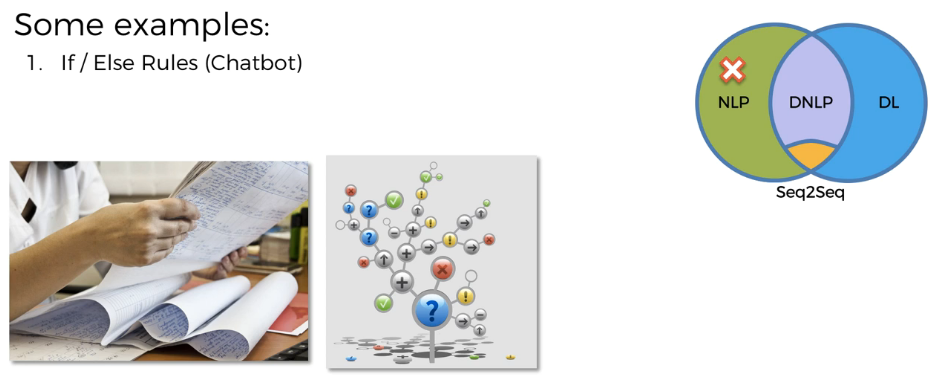
\includegraphics[width=0.8\linewidth,keepaspectratio]{nlp5}

\tiny{(Ref: Deep Learning and NLP A-Z - Kirill Eremenko)}
\end{center}
 Rule based chat-bot
	\begin{itemize}
	\item If/else rules
	\item Huge list of questions and answers
		\item Pattern based question-answers retrieval
		\item AIML (AI Markup language)
	\end{itemize}
	

\end{frame}

%%%%%%%%%%%%%%%%%%%%%%%%%%%%%%%%%%%%%%%%%%%%%%%%%%%%%%%%%%%
\begin{frame}[fragile]\frametitle{Traditional vs Deep NLP}
\begin{center}
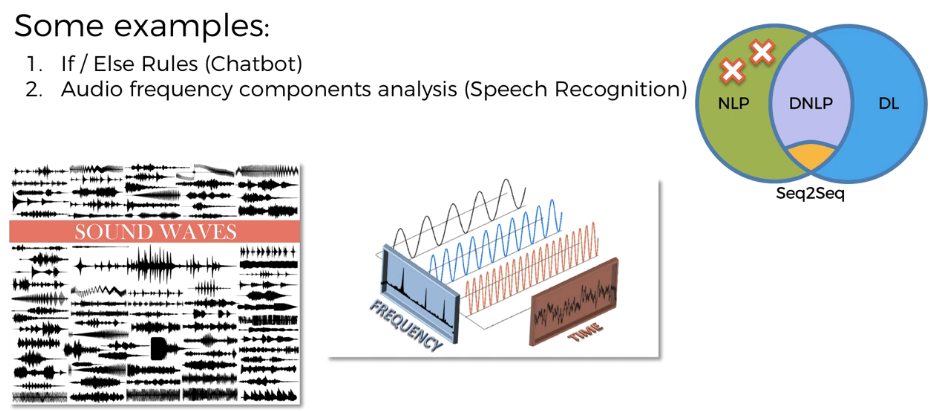
\includegraphics[width=0.8\linewidth,keepaspectratio]{nlp6}

\tiny{(Ref: Deep Learning and NLP A-Z - Kirill Eremenko)}
\end{center}
Speech Recognition
	\begin{itemize}
	\item Speech is matched to question speech, via frequency/signal matching
	\end{itemize}
	

\end{frame}

%%%%%%%%%%%%%%%%%%%%%%%%%%%%%%%%%%%%%%%%%%%%%%%%%%%%%%%%%%%
\begin{frame}[fragile]\frametitle{Traditional vs Deep NLP}
\begin{center}
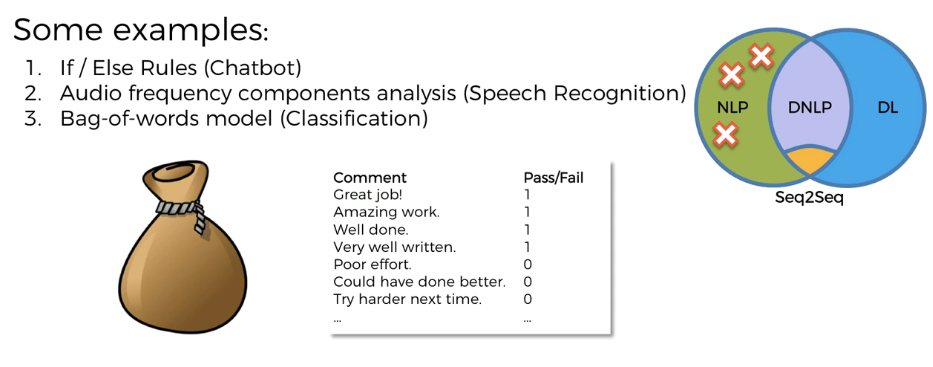
\includegraphics[width=0.8\linewidth,keepaspectratio]{nlp7}

\tiny{(Ref: Deep Learning and NLP A-Z - Kirill Eremenko)}
\end{center}
Bag of Words model
	\begin{itemize}
	\item Can be traditional as well as DNLP
	\item Frequencies of words is computed and based on positive and negative words (n-grams), classification can be done, either rule based or ML/DL way.
	\end{itemize}
\end{frame}

%%%%%%%%%%%%%%%%%%%%%%%%%%%%%%%%%%%%%%%%%%%%%%%%%%%%%%%%%%%
\begin{frame}[fragile]\frametitle{Traditional vs Deep NLP}
\begin{center}
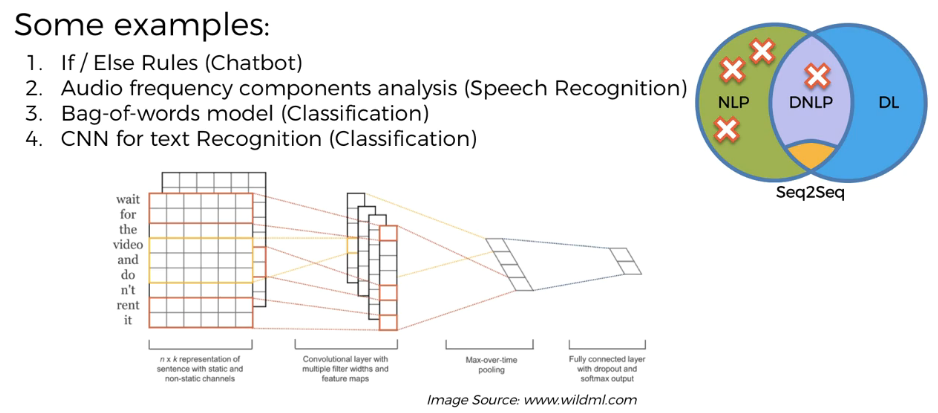
\includegraphics[width=0.8\linewidth,keepaspectratio]{nlp8}

\tiny{(Ref: Deep Learning and NLP A-Z - Kirill Eremenko)}
\end{center}
DNLP CNN 
	\begin{itemize}
	\item Convolution is slided through text, vertically, after they are brought into word vector form.
	\item Final NN does classification.
	\end{itemize}
\end{frame}

%%%%%%%%%%%%%%%%%%%%%%%%%%%%%%%%%%%%%%%%%%%%%%%%%%%%%%%%%%%
\begin{frame}[fragile]\frametitle{Traditional vs Deep NLP}
\begin{center}
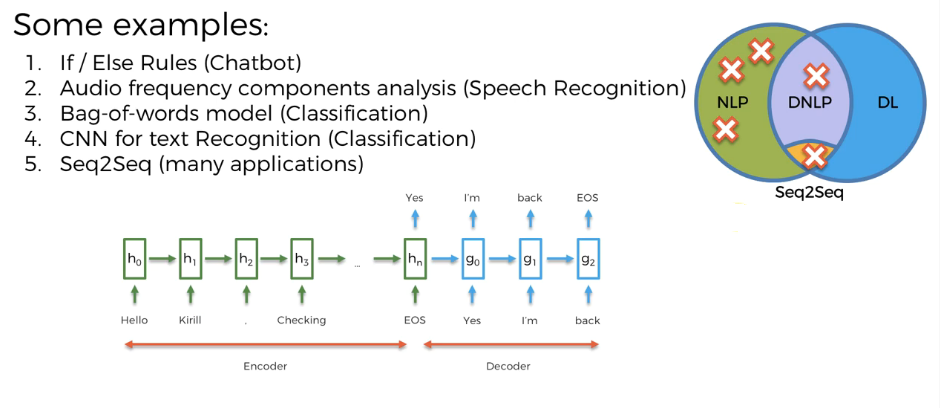
\includegraphics[width=0.8\linewidth,keepaspectratio]{nlp9}

\tiny{(Ref: Deep Learning and NLP A-Z - Kirill Eremenko)}
\end{center}
DNLP Seq2Seq 
	\begin{itemize}
	\item Sequence to Sequence modeling
	\item Translations, Q \& As.
	\end{itemize}
\end{frame}

%%%%%%%%%%%%%%%%%%%%%%%%%%%%%%%%%%%%%%%%%%%%%%%%%%%%%%%%%%%
\begin{frame}[fragile]\frametitle{Typical Machine Learning Classification}
	\begin{itemize}
	\item Questions are converted to bag of words (a vocab long vector, having frequency of specific words at their places)
		\item Each question thus gets converted to fixed size vector, which acts as list of features.
		\item In training, weights are computed based on the given target.
		\item Once model is ready, it is able to answer Yes or No to the question.
			\end{itemize}
\begin{center}
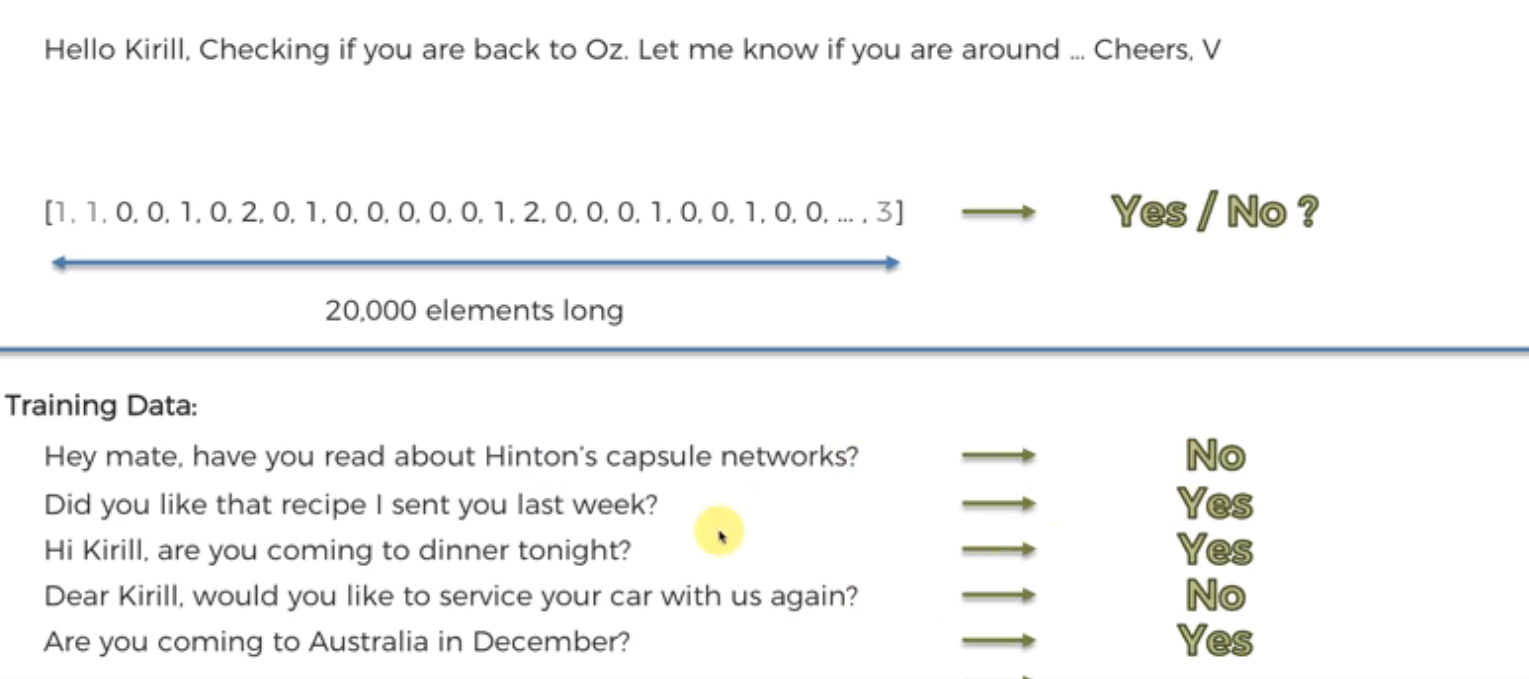
\includegraphics[width=0.6\linewidth,keepaspectratio]{nlp11}

\tiny{(Ref: Deep Learning and NLP A-Z - Kirill Eremenko)}
\end{center}

\end{frame}

%%%%%%%%%%%%%%%%%%%%%%%%%%%%%%%%%%%%%%%%%%%%%%%%%%%%%%%%%%%
\begin{frame}[fragile]\frametitle{ML DL}
As Logistic Regression (Machine Learning) you can use Neural Network (Deep Learning) to do the same job.

\begin{center}
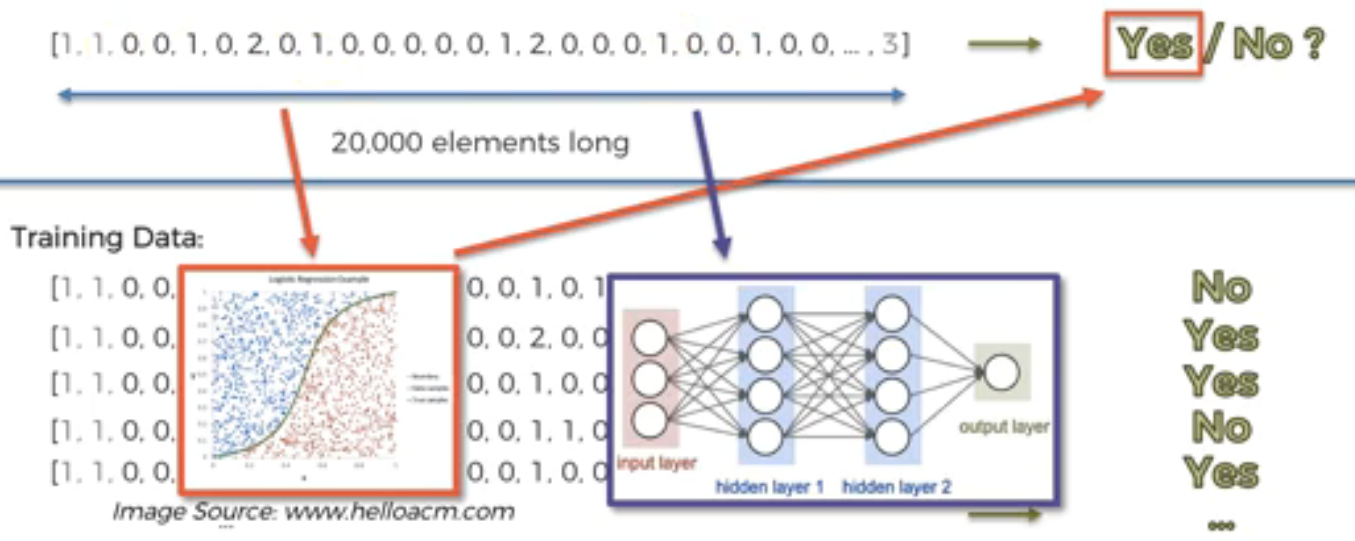
\includegraphics[width=\linewidth,keepaspectratio]{nlp12}

\tiny{(Ref: Deep Learning and NLP A-Z - Kirill Eremenko)}
\end{center}

\end{frame}

%%%%%%%%%%%%%%%%%%%%%%%%%%%%%%%%%%%%%%%%%%%%%%%%%%%%%%%%%%%
\begin{frame}[fragile]\frametitle{Issues with BoW model}
\begin{itemize}
\item Huge and sparse vectors for each sentence.
\item Does not take word order into account. Word before or after does not change the BoW vector. We are just counting the number of occurrences and NOT where they are.
\item Format is not flexible to have variable inputs and outputs.
\end{itemize}
			
Solution: Word embeddings and Seq2Seq architectures like RNN/LSTMs.

\end{frame}

%%%%%%%%%%%%%%%%%%%%%%%%%%%%%%%%%%%%%%%%%%%%%%%%%%%%%%%%%%%
\begin{frame}[fragile]\frametitle{Seq2Seq architecture}

\begin{center}
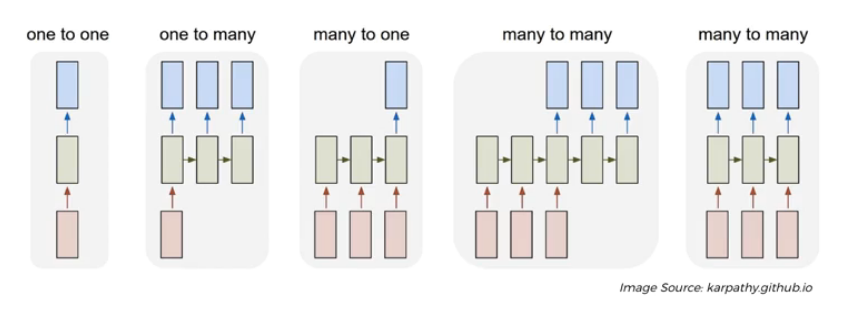
\includegraphics[width=\linewidth,keepaspectratio]{nlp13}

\tiny{(Ref: Deep Learning and NLP A-Z - Kirill Eremenko)}
\end{center}

For Seq2seq last 2 options are possible. We are going ahead with the 2nd last. Last one has fixed input and same size output.

\end{frame}

%%%%%%%%%%%%%%%%%%%%%%%%%%%%%%%%%%%%%%%%%%%%%%%%%%%%%%%%%%%
\begin{frame}[fragile]\frametitle{Seq2Seq architecture}

\begin{center}
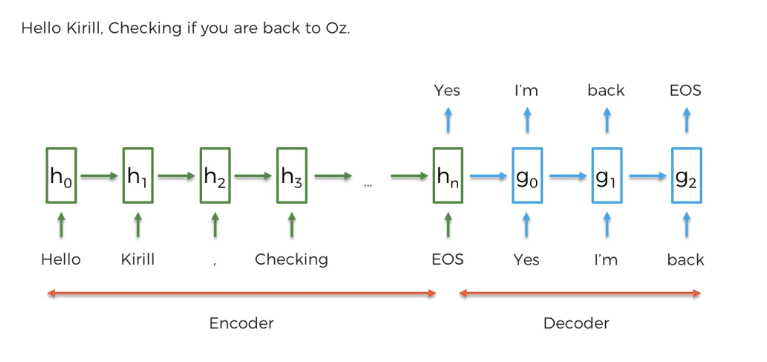
\includegraphics[width=0.8\linewidth,keepaspectratio]{nlp14}

\tiny{(Ref: Deep Learning and NLP A-Z - Kirill Eremenko)}
\end{center}
During training, Encoder is fed with Questions and decoder with Answers. Weights in gates, hidden states get settled. During testing for each sequence of input, encoder results in to a combo vector. Decoder takes this and starts spitting out words one by  one, probabilistically.

\end{frame}

%%%%%%%%%%%%%%%%%%%%%%%%%%%%%%%%%%%%%%%%%%%%%%%%%%%%%%%%%%%
\begin{frame}[fragile]\frametitle{Seq2Seq architecture}
It can get complex \ldots
\begin{center}
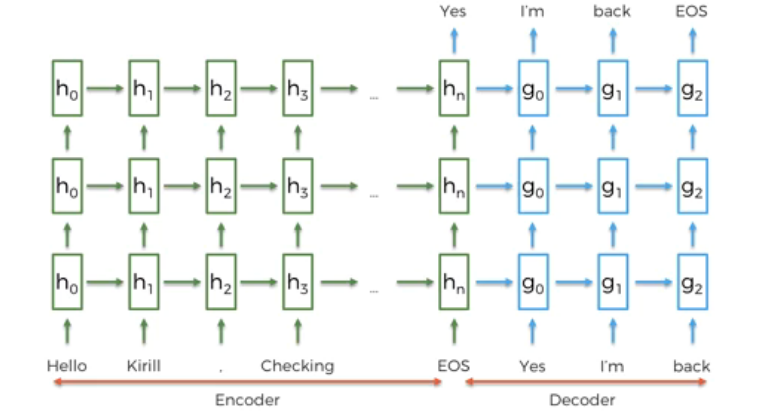
\includegraphics[width=0.8\linewidth,keepaspectratio]{nlp15}

\tiny{(Ref: Deep Learning and NLP A-Z - Kirill Eremenko)}
\end{center}

\end{frame}

%%%%%%%%%%%%%%%%%%%%%%%%%%%%%%%%%%%%%%%%%%%%%%%%%%%%%%%%%%%
\begin{frame}[fragile]\frametitle{Seq2Seq Training}

\begin{itemize}
\item Input: `` Did you like that recipe I sent you last week?''
\item Output: ``Yes it was great''.
\end{itemize}

\begin{center}
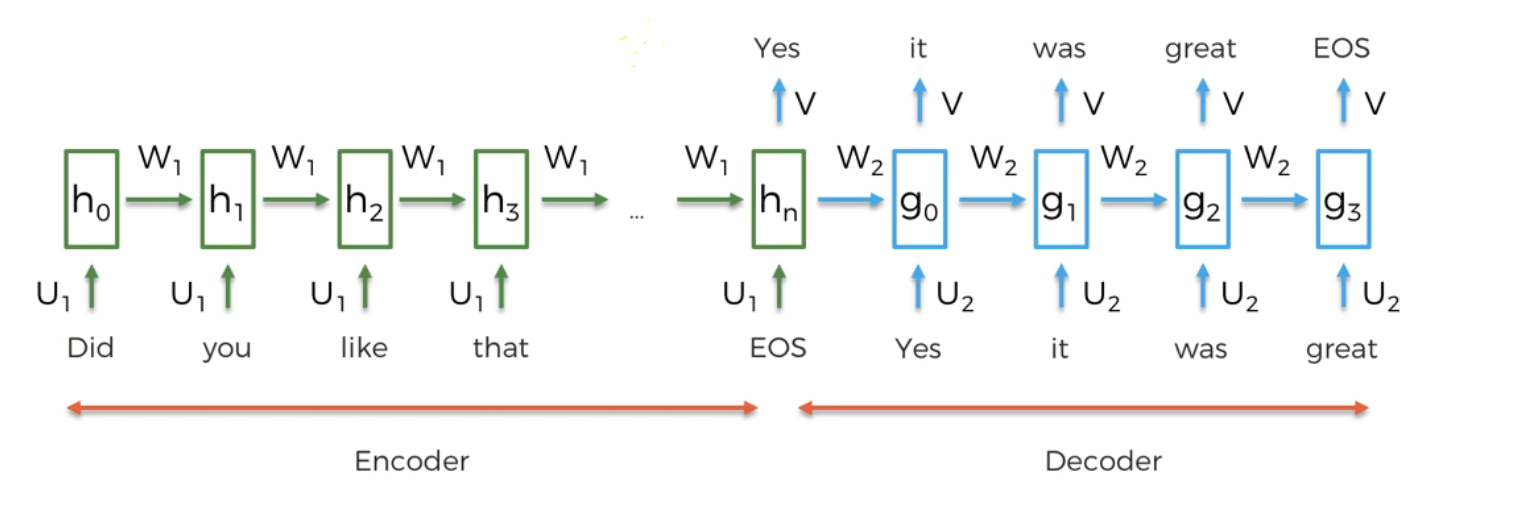
\includegraphics[width=0.8\linewidth,keepaspectratio]{nlp16}

\tiny{(Ref: Deep Learning and NLP A-Z - Kirill Eremenko)}
\end{center}
Parameters that get optimized during training are:
\begin{itemize}
\item $U_1$ : Input weights per word  Encoder.
\item $U_2$ : Decoder weight for input, which is previous word.
\item $V$: Decoder Prediction/Output.
\item $W_1$ :  Encoder weights.
\item $W_2$ :  Decoder weights.
\end{itemize}


\end{frame}

%%%%%%%%%%%%%%%%%%%%%%%%%%%%%%%%%%%%%%%%%%%%%%%%%%%%%%%%%%%
\begin{frame}[fragile]\frametitle{Attention Mechanism}

\begin{itemize}
\item A single meaning/context vector ($h_n$), the final encoder vector, to carry whole sentence is too much to expect!!!
\item We need luxury of looking back at source, whenever needed.
\item Input Question:`` How is your sister?''
\item Output Answer: ``Thank you, she is fine.''
\end{itemize}
\begin{center}
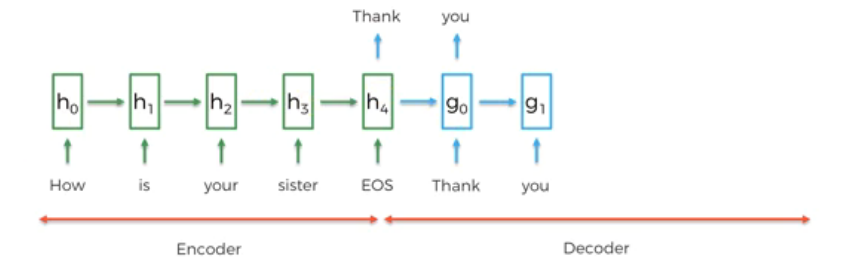
\includegraphics[width=0.8\linewidth,keepaspectratio]{nlp19}

\tiny{(Ref: Deep Learning and NLP A-Z - Kirill Eremenko)}
\end{center}

\end{frame}

%%%%%%%%%%%%%%%%%%%%%%%%%%%%%%%%%%%%%%%%%%%%%%%%%%%%%%%%%%%
\begin{frame}[fragile]\frametitle{Attention Mechanism}

\begin{itemize}
\item Say, at the 3rd decoded word, we need to look back (ie Attention).
\item Through training, decoder will know, for a particular word, which of the input words need to be looked at.
\item That source word has highest weight (all learned through training)
\item Element wise product of h vectors and weights is fed into the $g_1$ cell as additional input. Thats context vector (w attention)
\end{itemize}
\begin{center}
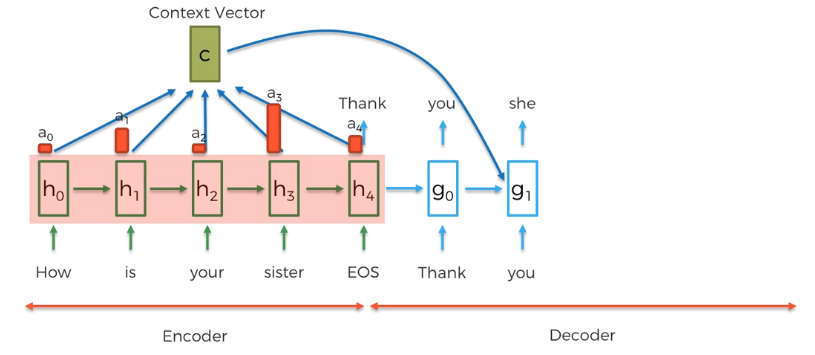
\includegraphics[width=0.6\linewidth,keepaspectratio]{nlp20}

\tiny{(Ref: Deep Learning and NLP A-Z - Kirill Eremenko)}
\end{center}

\end{frame}

%%%%%%%%%%%%%%%%%%%%%%%%%%%%%%%%%%%%%%%%%%%%%%%%%%%%%%%%%%%
\begin{frame}[fragile]\frametitle{Attention Mechanism}

\begin{itemize}
\item We need to find pronoun for the answer , ``he or she is fine''
\item Need to find noun in the question, here its ``sister''. So ``she'' is picked.
\item Thats why the higher weight comes.
\item Other words may also be needed, as per their weights.
\end{itemize}
\begin{center}
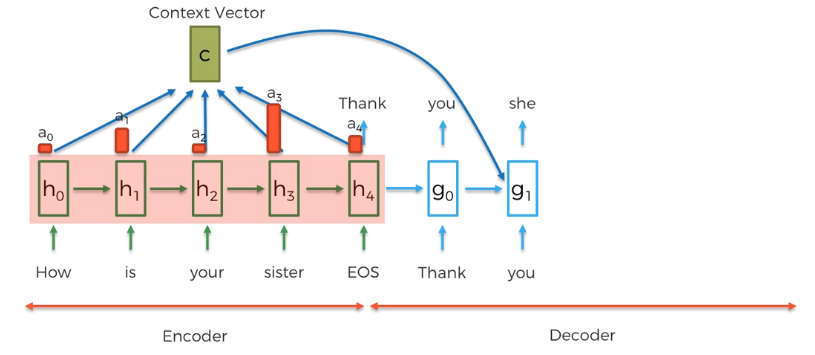
\includegraphics[width=0.6\linewidth,keepaspectratio]{nlp20}

\tiny{(Ref: Deep Learning and NLP A-Z - Kirill Eremenko)}
\end{center}

\end{frame}


%%%%%%%%%%%%%%%%%%%%%%%%%%%%%%%%%%%%%%%%%%%%%%%%%%%%%%%%%%%
\begin{frame}[fragile]\frametitle{Attention Mechanism}

\begin{itemize}
\item Next word after ``she''?
\item A new context vector. Highest is ``is'', using which we will find correct verb.
\item Plural or singular is decided by $a_4$ weight.
\end{itemize}
\begin{center}
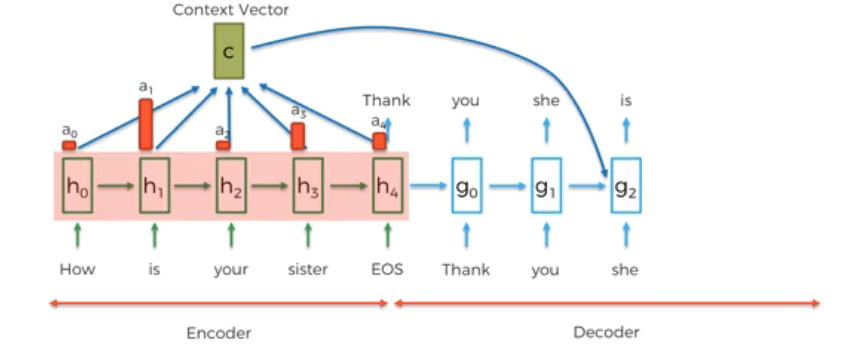
\includegraphics[width=0.6\linewidth,keepaspectratio]{nlp21}

\tiny{(Ref: Deep Learning and NLP A-Z - Kirill Eremenko)}
\end{center}

\end{frame}



%%%%%%%%%%%%%%%%%%%%%%%%%%%%%%%%%%%%%%%%%%%%%%%%%%%%%%%%%%%
\begin{frame}[fragile]\frametitle{Greedy Decoding vs Beam Search Decoding}
Greedy Decoding
\begin{itemize}
\item Given context vector, it gives out the word with max probability out of whole vocab
\item Then with this as input, along with the passed-along vector, find another word with max probability.
\item At the end, it spits out EOS.
\item Its greedy as it picks max probability at each time step.
\end{itemize}
\begin{center}
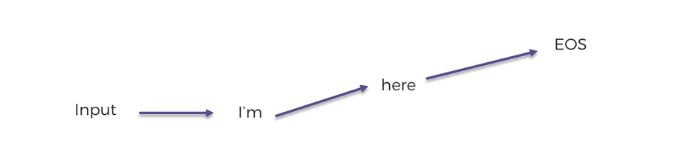
\includegraphics[width=0.8\linewidth,keepaspectratio]{nlp17}

\tiny{(Ref: Deep Learning and NLP A-Z - Kirill Eremenko)}
\end{center}

\end{frame}

%%%%%%%%%%%%%%%%%%%%%%%%%%%%%%%%%%%%%%%%%%%%%%%%%%%%%%%%%%%
\begin{frame}[fragile]\frametitle{Greedy Decoding vs Beam Search Decoding}
Beam Search Decoding
\begin{itemize}
\item More sophisticated. Instead of looking at the word with MAX probability, we look at top 3.
\item We have now 3 versions of sequences starting with these 3 start words.
\item Its repeated at each level, like a tree.
\item Winner is picked at max joint probability.
\end{itemize}
\begin{center}
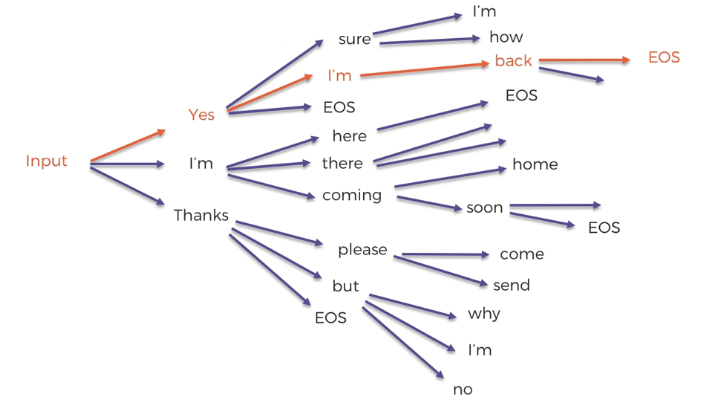
\includegraphics[width=0.6\linewidth,keepaspectratio]{nlp18}

\tiny{(Ref: Deep Learning and NLP A-Z - Kirill Eremenko)}
\end{center}

\end{frame}

